%% Template file for all Software/Hardware modules

% Replace "Name of Module" with the name of this module
\chapter{Software Design Overview}

\section{Description}

The POWER project uses various pieces of software to control the Satellites, provide an API for displays, and generate pages for the primary display. The POWER project will consist of the following pieces of software:
\begin{itemize}
 \item The microprocessor code
 \item The server code to communicate with the Satellites
 \item The server code to present the API
 \item The client code to render the display for the user
\end{itemize}

The microprocessor code is documented in the hardware section because it is very related to the hardware, and it is much more logical to put the  code there.

\subsection{The Display Backend}

The general plan for the backend is to write modules for a Django web application. This modules will either be running in the background and reporting to the through the REST API functions, or responding to user requests.

The logic for using Django as the base, and write modules around Django, is one of necessity. We do not have enough time or manpower to make everything we need from scratch. Therefore, we will be using several open source utilities to assist us. 

Django will give us an easy-to-use database interface. It will deal with sanitizing all SQL queries, and make sure all output is escaped (ie, no XSS). Using Django gives us almost all of the security benefits listed in our non-functional requirements.

To make our REST API, we will utilize an open-source Django library called tastypie. Tastypie gives us both model resources (that is, api elements that are basically the database tables) and the ability to create custom resources that may, or may not, map to the database. The one (that's right, one) instance where we may not want to directly map something to the database is when we are looking at turning the outlets on and off.

Another advantage of Django is that is comes with a very extensive, expandable, and adaptable authentication system. This will help accomplish several optional and required features almost instantly. 

\subsection{The Display Frontend}

The general plan for the frontend is to serve up some fairly static pages, and uses extensive amounts of Javascript to fill in the content and animate things. The frontend will communicate with the backend through the REST API.

\section{Program Flow}

This program will have three main "threads". One thread would be responsible for listening to messages from the Satellites, and another would be responsible for listening and responding to requests on the API. The last thread would be responsible for serving up static files for the main display.

The Satellite thread will be responsible for taking the logging information provided by the Satellites and storing it in the database. Each Satellite will report it's information to the server once every second. Therefore, all this thread needs to do is react to incoming connections.

The API thread would provide the Representation State Transfer API (REST) that will be used by all future displays to get data in a standardized, well defined way. This thread will NOT be serving up images or page templates. This is done to make best use of the caching functionality included in the HTTP server software that will be used.

The last thread will be running a "dumb" web page that servers up static HTML and Javascript files. This thread will also retrieve images and CSS files from the server.

\section{Data Flow}

This application will use a SQL database to store all data. Each module will interact with the REST API, which interacts with the database as needed. The diagram for this database is broken down in the "Sub-modules" section, with a diagram for each logical grouping of tables.

\begin{figure}
\centering
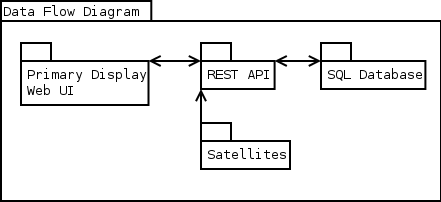
\includegraphics[scale=0.5]{Software/images/DataFlowDiagram.png}
\caption{Data Flow Diagram}
\label{DataFlowDiagram}
\end{figure}

Figure \ref{DataFlowDiagram} shows how various components will be interacting. Notice that the database is not directly accessed by any components, but goes the a REST API instead. This allows us to provide a standard interface should be more-or-less accessible from any programming language or system. This will also allow us to use some well-known security features, such as TLS.

\section{UML Diagrams}

% Any diagrams that can describe the system design
%  Such as inheritance and actors

\section{Potential Problems}

% A list of potentional programs along with suggestions
%  on ways to work around them. Elaborate on why the problem
%  exists

\section{Sub-modules 1}

% This is a second section of modules,
%  and should consists of this module broken 
%  down further into components

